% Seed ensembles slide. Build: pdflatex seed_slide.tex  (needs seed_ensembles_uplift.pdf from ../slide_seed_chart.py)
\documentclass[aspectratio=169,10pt]{beamer}
\usetheme{default}
\setbeamertemplate{navigation symbols}{}
\setbeamerfont{frametitle}{size=\large,series=\bfseries}
\setbeamercolor{frametitle}{fg=black}
\usepackage{tikz}
\usetikzlibrary{positioning,calc,arrows.meta,decorations.pathreplacing,fit}
\usepackage{graphicx}

\definecolor{sys}{HTML}{D9D8D3}
\definecolor{ex}{HTML}{CDE2FB}
\definecolor{test}{HTML}{FBE3C9}
\definecolor{seedA}{HTML}{E87BA4}
\definecolor{seedB}{HTML}{1BAF7A}
\definecolor{seedC}{HTML}{4A3AA7}
\definecolor{dots}{HTML}{1BAF7A}
\definecolor{ink}{HTML}{52514E}

% one seeded row: #1 y, #2 seed colour, #3 seed text, #4 name
  \newcommand{\row}[4]{% #1 y, #2 seed colour, #3 seed text, #4 name
    \node[blk, fill=sys, minimum width=12mm] (s#4) at (0,#1) {system};
    \node[blk, fill=#2!30, draw=#2, minimum width=17mm, right=0pt of s#4] (k#4) {#3};
    \node[blk, fill=ex, minimum width=30mm, right=0pt of k#4] (e#4) {10 worked examples};
    \node[blk, fill=test, minimum width=33mm, right=0pt of e#4] (t#4) {question\ \ \texttt{Filler:}\ \ \texttt{Answer:}};
    \node[blk, fill=test, minimum width=8mm, right=0pt of t#4, font=\tiny\ttfamily] (a#4) {</think>};
  }
\begin{document}
\begin{frame}[t]{Random-text ``seeds'' instead of filler: ensembling over contexts}
\vspace{-3mm}
\centering

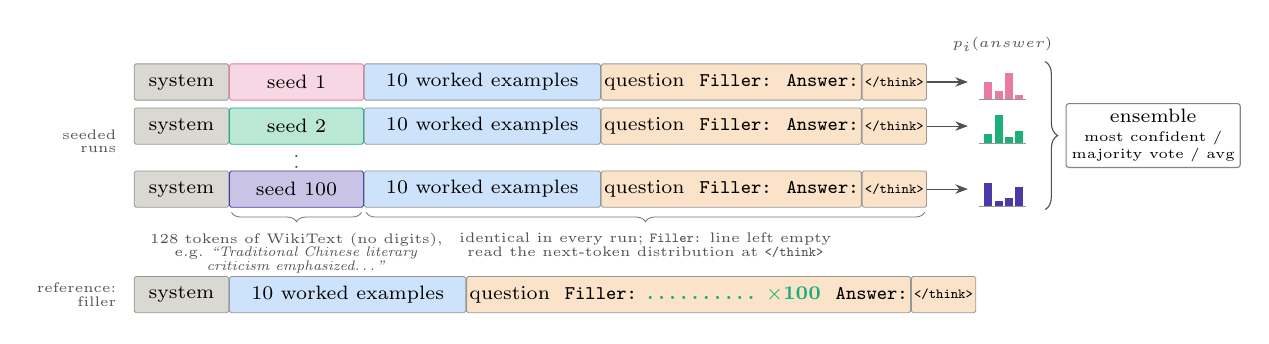
\begin{tikzpicture}[
  font=\scriptsize, >={Stealth[length=1.6mm]},
  blk/.style={draw=ink!60, line width=0.3pt, minimum height=4.6mm, inner sep=1pt, anchor=west, rounded corners=0.6pt},
  lab/.style={font=\tiny, text=ink},
]
  \row{0}{seedA}{seed 1}{1}
  \row{-5.6mm}{seedB}{seed 2}{2}
  \node[font=\scriptsize, text=ink] at ($(k2.south)+(0,-1.9mm)$) {$\vdots$};
  \row{-13.6mm}{seedC}{seed 100}{3}

  % per-seed answer distributions (mini bars)
  \foreach \r/\c/\h in {1/seedA/{2.2,1.0,3.4,0.6}, 2/seedB/{1.2,3.6,0.8,1.6}, 3/seedC/{3.0,0.7,1.1,2.4}}{
    \begin{scope}[shift={($(a\r.east)+(6mm,-2.2mm)$)}]
      \foreach \v [count=\i] in \h { \fill[\c] (\i*1.3mm,0) rectangle ++(1mm,\v mm); }
      \draw[ink!60, line width=0.2pt] (0.6mm,0) -- (6.6mm,0);
    \end{scope}
    \draw[->, ink] (a\r.east) -- ++(5.2mm,0);
  }
  \node[lab, anchor=south] at ($(a1.east)+(9.6mm,2.6mm)$) {$p_i(\text{answer})$};

  % brace + ensemble
  \draw[decorate, decoration={brace, amplitude=1.6mm}, ink, line width=0.4pt]
    ($(a1.east)+(15mm,2.6mm)$) -- ($(a3.east)+(15mm,-2.6mm)$) coordinate[midway] (br);
  \node[draw=ink!70, rounded corners=1pt, fill=white, font=\scriptsize, align=center, inner sep=2pt, anchor=west]
    (ens) at ($(br)+(2.6mm,0)$) {ensemble\\[-0.4ex]{\tiny most confident /}\\[-0.6ex]{\tiny majority vote / avg}};

  % braces naming the parts
  \draw[decorate, decoration={brace, amplitude=1.2mm, mirror}, ink!80, line width=0.3pt]
    ($(k3.south west)+(0.3mm,-0.6mm)$) -- ($(k3.south east)+(-0.3mm,-0.6mm)$) node[midway, below=1.4mm, lab, align=center]{128 tokens of WikiText (no digits),\\[-0.5ex]e.g.\ \emph{``Traditional Chinese literary}\\[-0.5ex]\emph{criticism emphasized\ldots''}};
  \draw[decorate, decoration={brace, amplitude=1.2mm, mirror}, ink!80, line width=0.3pt]
    ($(e3.south west)+(0.3mm,-0.6mm)$) -- ($(a3.south east)+(-0.3mm,-0.6mm)$) node[midway, below=1.4mm, lab, align=center]{identical in every run; \texttt{Filler:} line left empty\\[-0.5ex]read the next-token distribution at \texttt{</think>}};

  % reference row: 100 dots
  \node[blk, fill=sys, minimum width=12mm] (sd) at (0,-27mm) {system};
  \node[blk, fill=ex, minimum width=30mm, right=0pt of sd] (ed) {10 worked examples};
  \node[blk, fill=test, minimum width=50mm, right=0pt of ed] (td) {question\ \ \texttt{Filler:} {\color{dots}\textbf{.\,.\,.\,.\,.\,.\,.\,.\,.\,. $\times$100}}\ \ \texttt{Answer:}};
  \node[blk, fill=test, minimum width=8mm, right=0pt of td, font=\tiny\ttfamily] (ad) {</think>};
  \node[lab, anchor=east, align=right] at ($(sd.west)+(-1mm,0)$) {reference:\\[-0.5ex]filler};
  \node[lab, anchor=east, align=right] at ($(s1.west)+(-1mm,-7.5mm)$) {seeded\\[-0.5ex]runs};
\end{tikzpicture}

\vspace{0mm}
\begin{minipage}[t]{0.55\textwidth}
  \vspace{0pt}
  \includegraphics[width=\linewidth]{seed_ensembles_uplift.pdf}
\end{minipage}\hfill
\begin{minipage}[t]{0.42\textwidth}
  \vspace{1mm}
  \scriptsize
  \textbf{Most confident seed.} Run all $n$ seeded prompts; keep the one whose top answer has the highest probability, and use its answer distribution. Needs no label.

  \smallskip
  \textbf{Majority vote.} Take each seeded run's greedy (argmax) answer; output the most common one.

  \smallskip
  \textbf{Takeaway} (uplift over no filler, 100 seeds). One seed: +0.4 points. Averaging: +1.6. \emph{Selecting} the most confident seed: +9.6, i.e.\ 63\% of the 100-dot uplift (+15.2). Majority vote: +4.2 greedy, 37\% of the dots' +11.2.

  \smallskip
  {\tiny\color{ink} DeepSeek V4 Flash, 10-shot, 598 variable-binding problems. Uplift = method $-$ no filler on the same problem (paired), in points; \% = share of the 100-dot uplift. T=1: P(correct answer) within the number distribution; ensembles over the first $n$ of 100 seeds; bars $\pm$1 SE.}
\end{minipage}
\end{frame}
\end{document}
